\section{実験装置}

\subsection{作用力測定装置}
本研究において使用した作用力装置の写真をFig.1に示す.
回流水槽を用いた作用力測定実験の際に使用する作用力測定装置を
性能評価実験を行うため,製作したフレームに組み付けた.
また,本研究において評価対象となるひずみセンサの取付部を(b)に,
作用力を与えるタイヤモデルの取付部を(c)に示している.

\begin{figure}[htbp]
    \begin{minipage}[b]{0.48\linewidth}
        \centering
        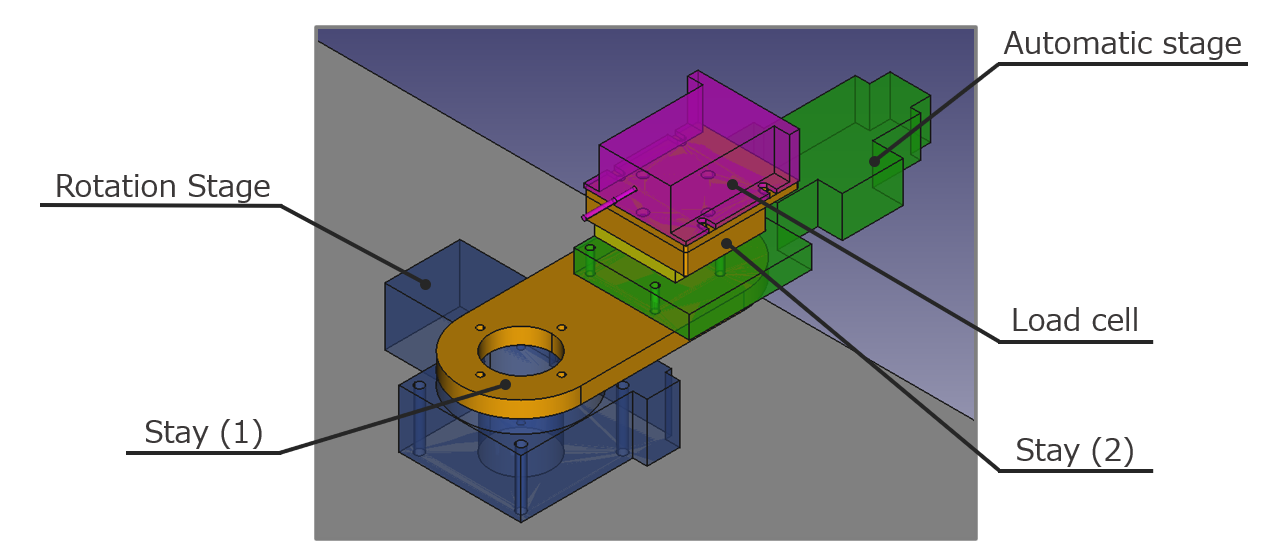
\includegraphics[width=70mm]{images/21-1.png}
        \subcaption{Overall photograph}
    \end{minipage}
    \begin{minipage}[b]{0.42\linewidth}
        \centering
        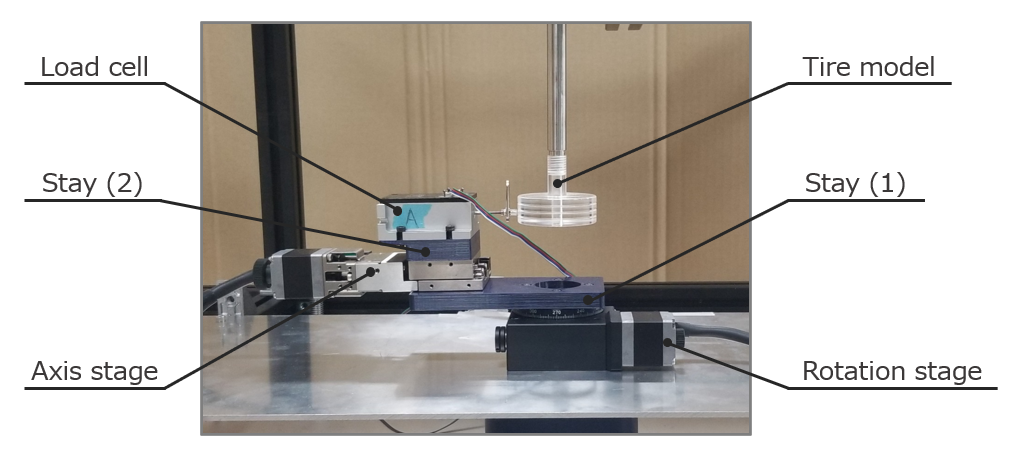
\includegraphics[width=45mm]{images/21-2.png}
        \subcaption{Mounting part of strain sensors}
        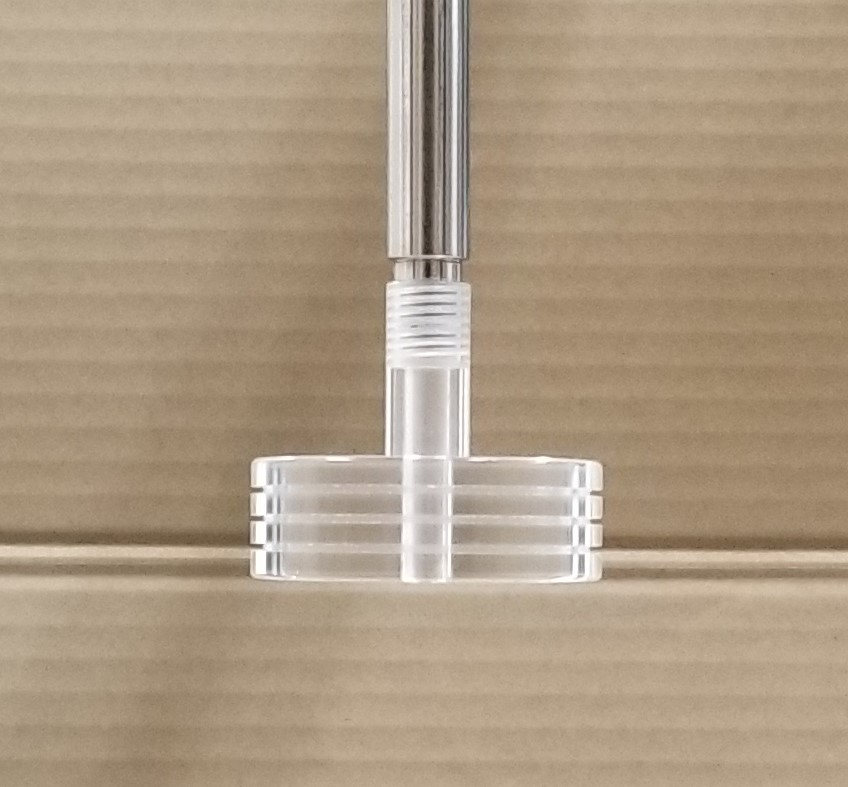
\includegraphics[width=45mm]{images/21-3.png}
        \subcaption{Mounting part of tire model}
    \end{minipage}
    \caption{Acting force measuring device}
\end{figure}

\newpage

\subsubsection{測定原理}

Fig.1の作用力測定装置のひずみ計測方法には,2ゲージ法を採用している.
また,ひずみセンサはKYOWA製の短軸半導体ひずみセンサ(KSPB-2-120)を使用しており,
一般のひずみセンサのゲージ率が2 $[\Omega]$ 程度であることに比べて
使用した半導体ひずみセンサはゲージ率が 120 $[\Omega]$ 程度と
非常に大きいという特徴がある.これは,回流水槽を用いた作用力測定実験において,
作用力によって生じるひずみを曲げひずみとして測定し,
そのひずみ量は非常に小さいことから,これを測定するためにゲージ率の大きい
高感度の半導体ひずみセンサを使用し,2ゲージ法によってひずみセンサ単体の場合に比べて,
2倍の出力電圧を得ることができるためである.
したがって,作用力測定装置に加わる微小なひずみを測定することを目的としており,
作用力測定実験に適した測定方法であるといえる.

\subsection{校正実験装置}
本研究において製作・使用した実験装置の概略図および写真をFig.2に示す.

\begin{figure}[htbp]
    \begin{center}
        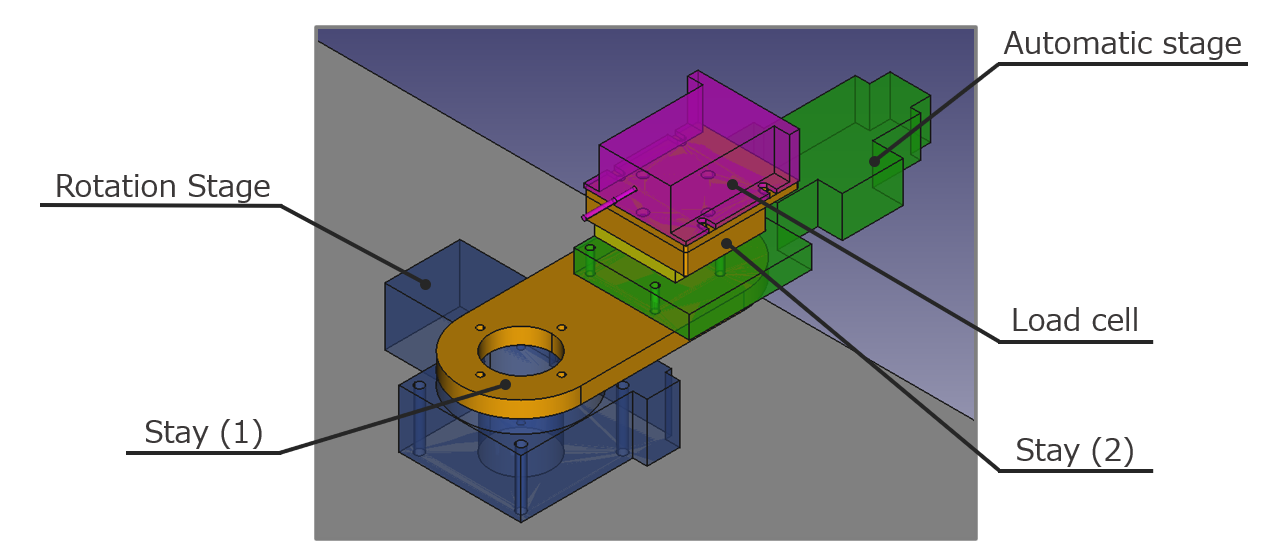
\includegraphics[width=110mm]{images/22-1.png}
        \subcaption{3D CAD}
        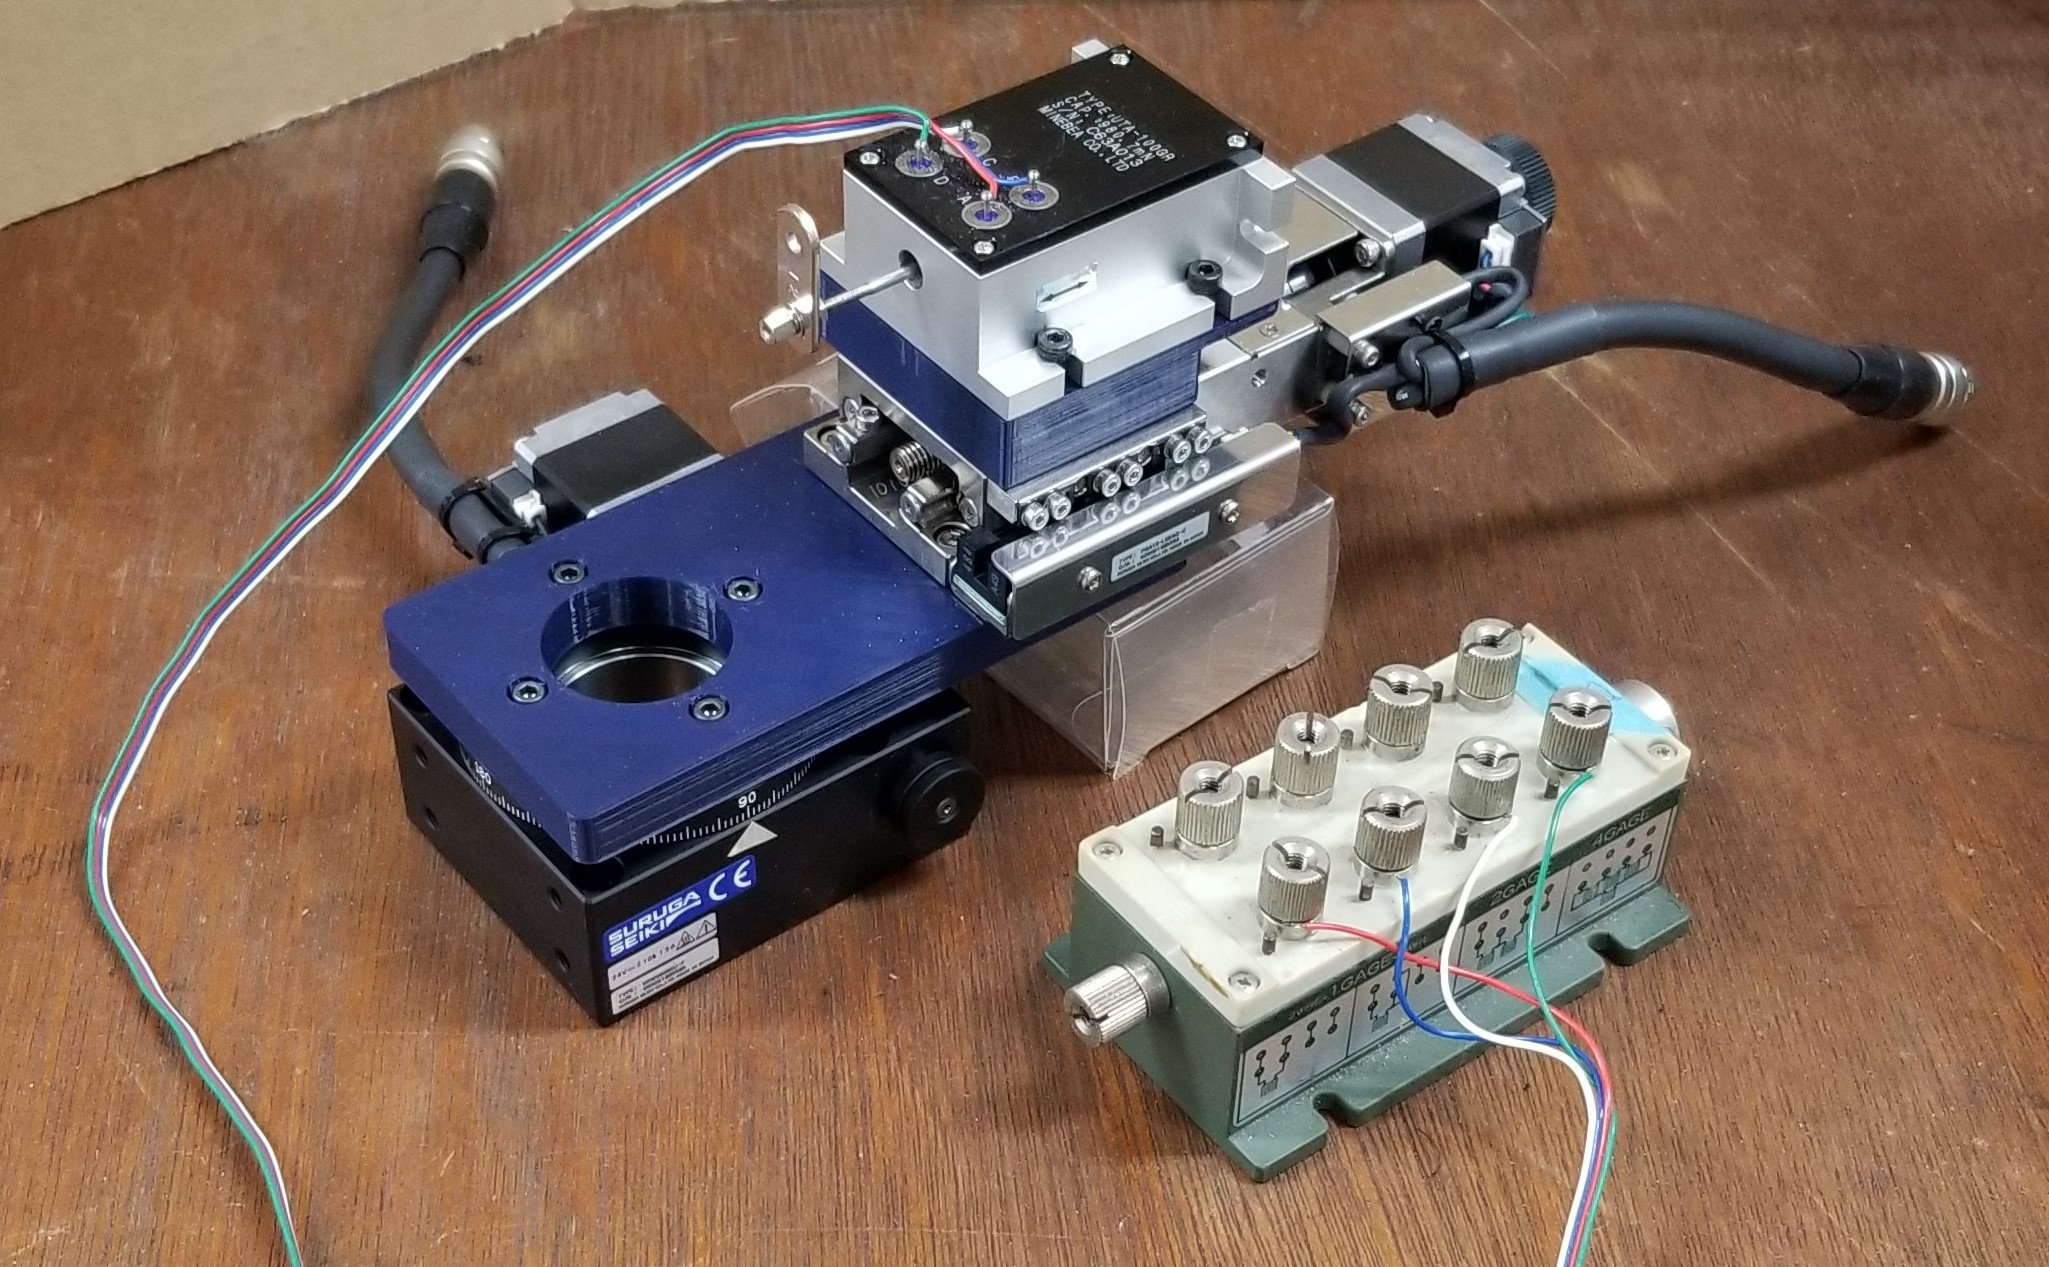
\includegraphics[width=75mm]{images/22-2.png}
        \subcaption{Photograph}
    \end{center}
    \caption{Calibration device}
\end{figure}

\newpage

校正装置は,作用力測定装置に取り付けられた2組のひずみセンサについて,
作用力の角度による出力電圧の関係性を調べる目的がある.
また,自動ステージを用いて人為的な操作を可能な限り減らし自動化することで,
不本意なノイズの削減や複数回の実験を効率的に行うことができた.
Fig.2に示す作用力を与える校正装置は,自動一軸ステージ,自動回転ステージ,ロードセル,
それらを接続するステーから構成される.

また,Fig.3に示すように作用力測定装置のフレームに校正実験装置を取り付けることで,
作用力測定と校正実験装置の位置関係を保持することができる.
校正実験装置はアルミ板を介してフレームに取り付ける.
設置の際には,作用力測定装置をフレーム上に設置し,
作用力測定装置の回転軸と自動回転ステージの回転軸を
できるだけ一致させるように調整をしながら行うことが好ましい.
\begin{figure}[htbp]
    \footnotesize
    \begin{center}
        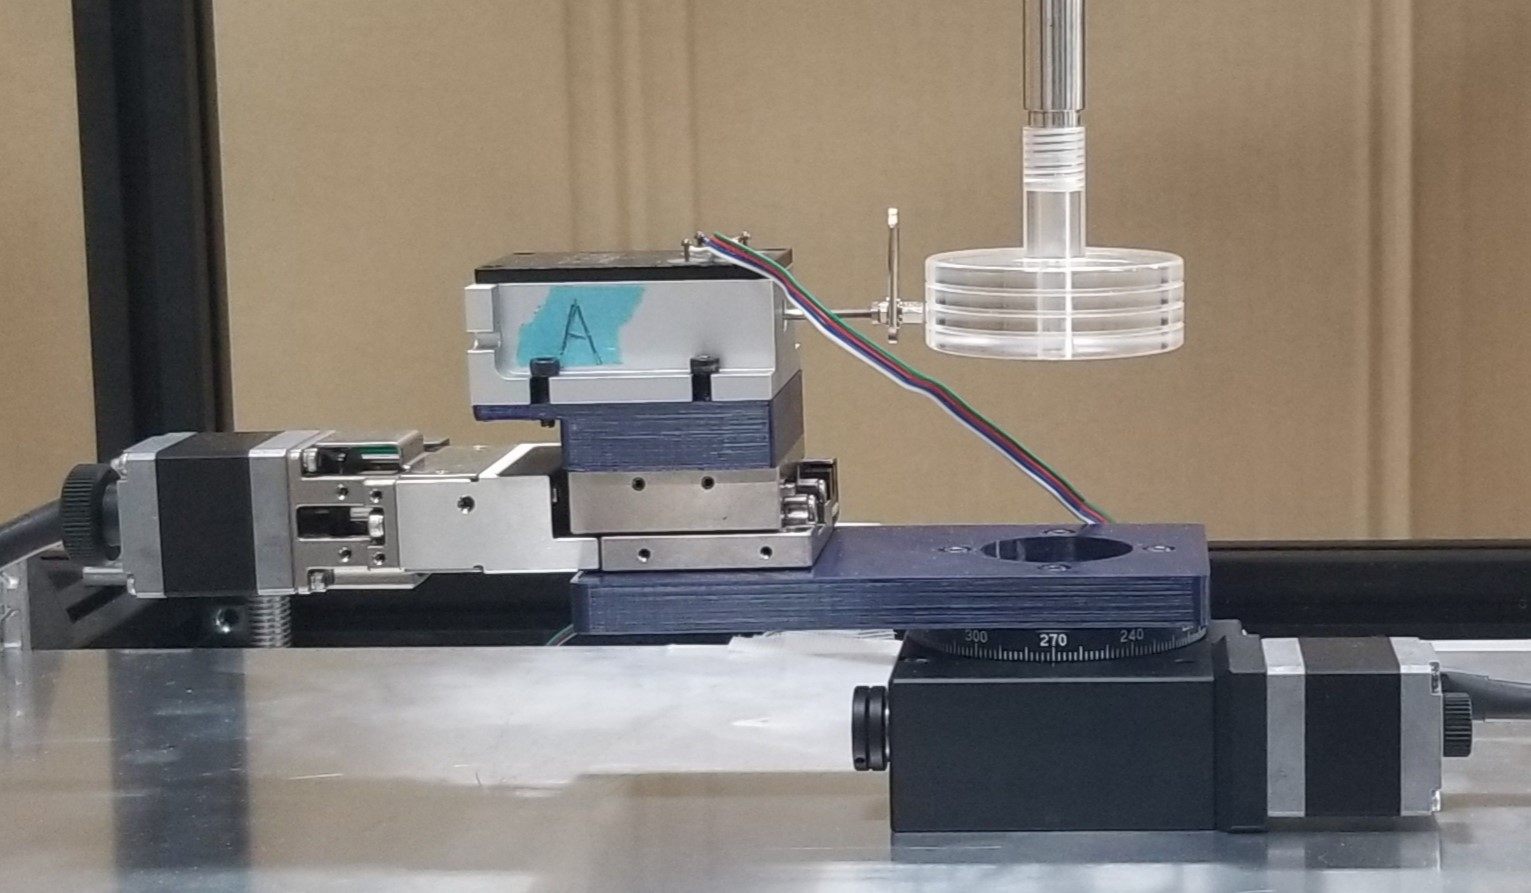
\includegraphics[width=75mm]{images/22-3.png}
        \caption{Assembled calibaration device}
    \end{center}
\end{figure}

なお,本研究では,ロードセルはミネベアミツミ製 微小荷重引張圧縮型 UTA (UTA-100GR),
自動一軸ステージは駿河精機製 リニアボールガイドステージ (PG530),
自動回転ステージは駿河精機製 回転ステージ ウォームギア (KRW06360),
自動ステージコントローラはFig.4に示す駿河精機製 ステッピングモータコントローラ(DS102MS) を使用している.
また,2つのステーについては,自動回転ステージ上に取り付けることになり,
軽量である必要があるため3Dプリンタを用いて製作し,使用している.
% ジョイントの形状や材料の充填率を
% 変更しながら重量と剛性のバランスを調整しながら製作を行った.

\begin{figure}[htbp]
    \footnotesize
    \begin{center}
        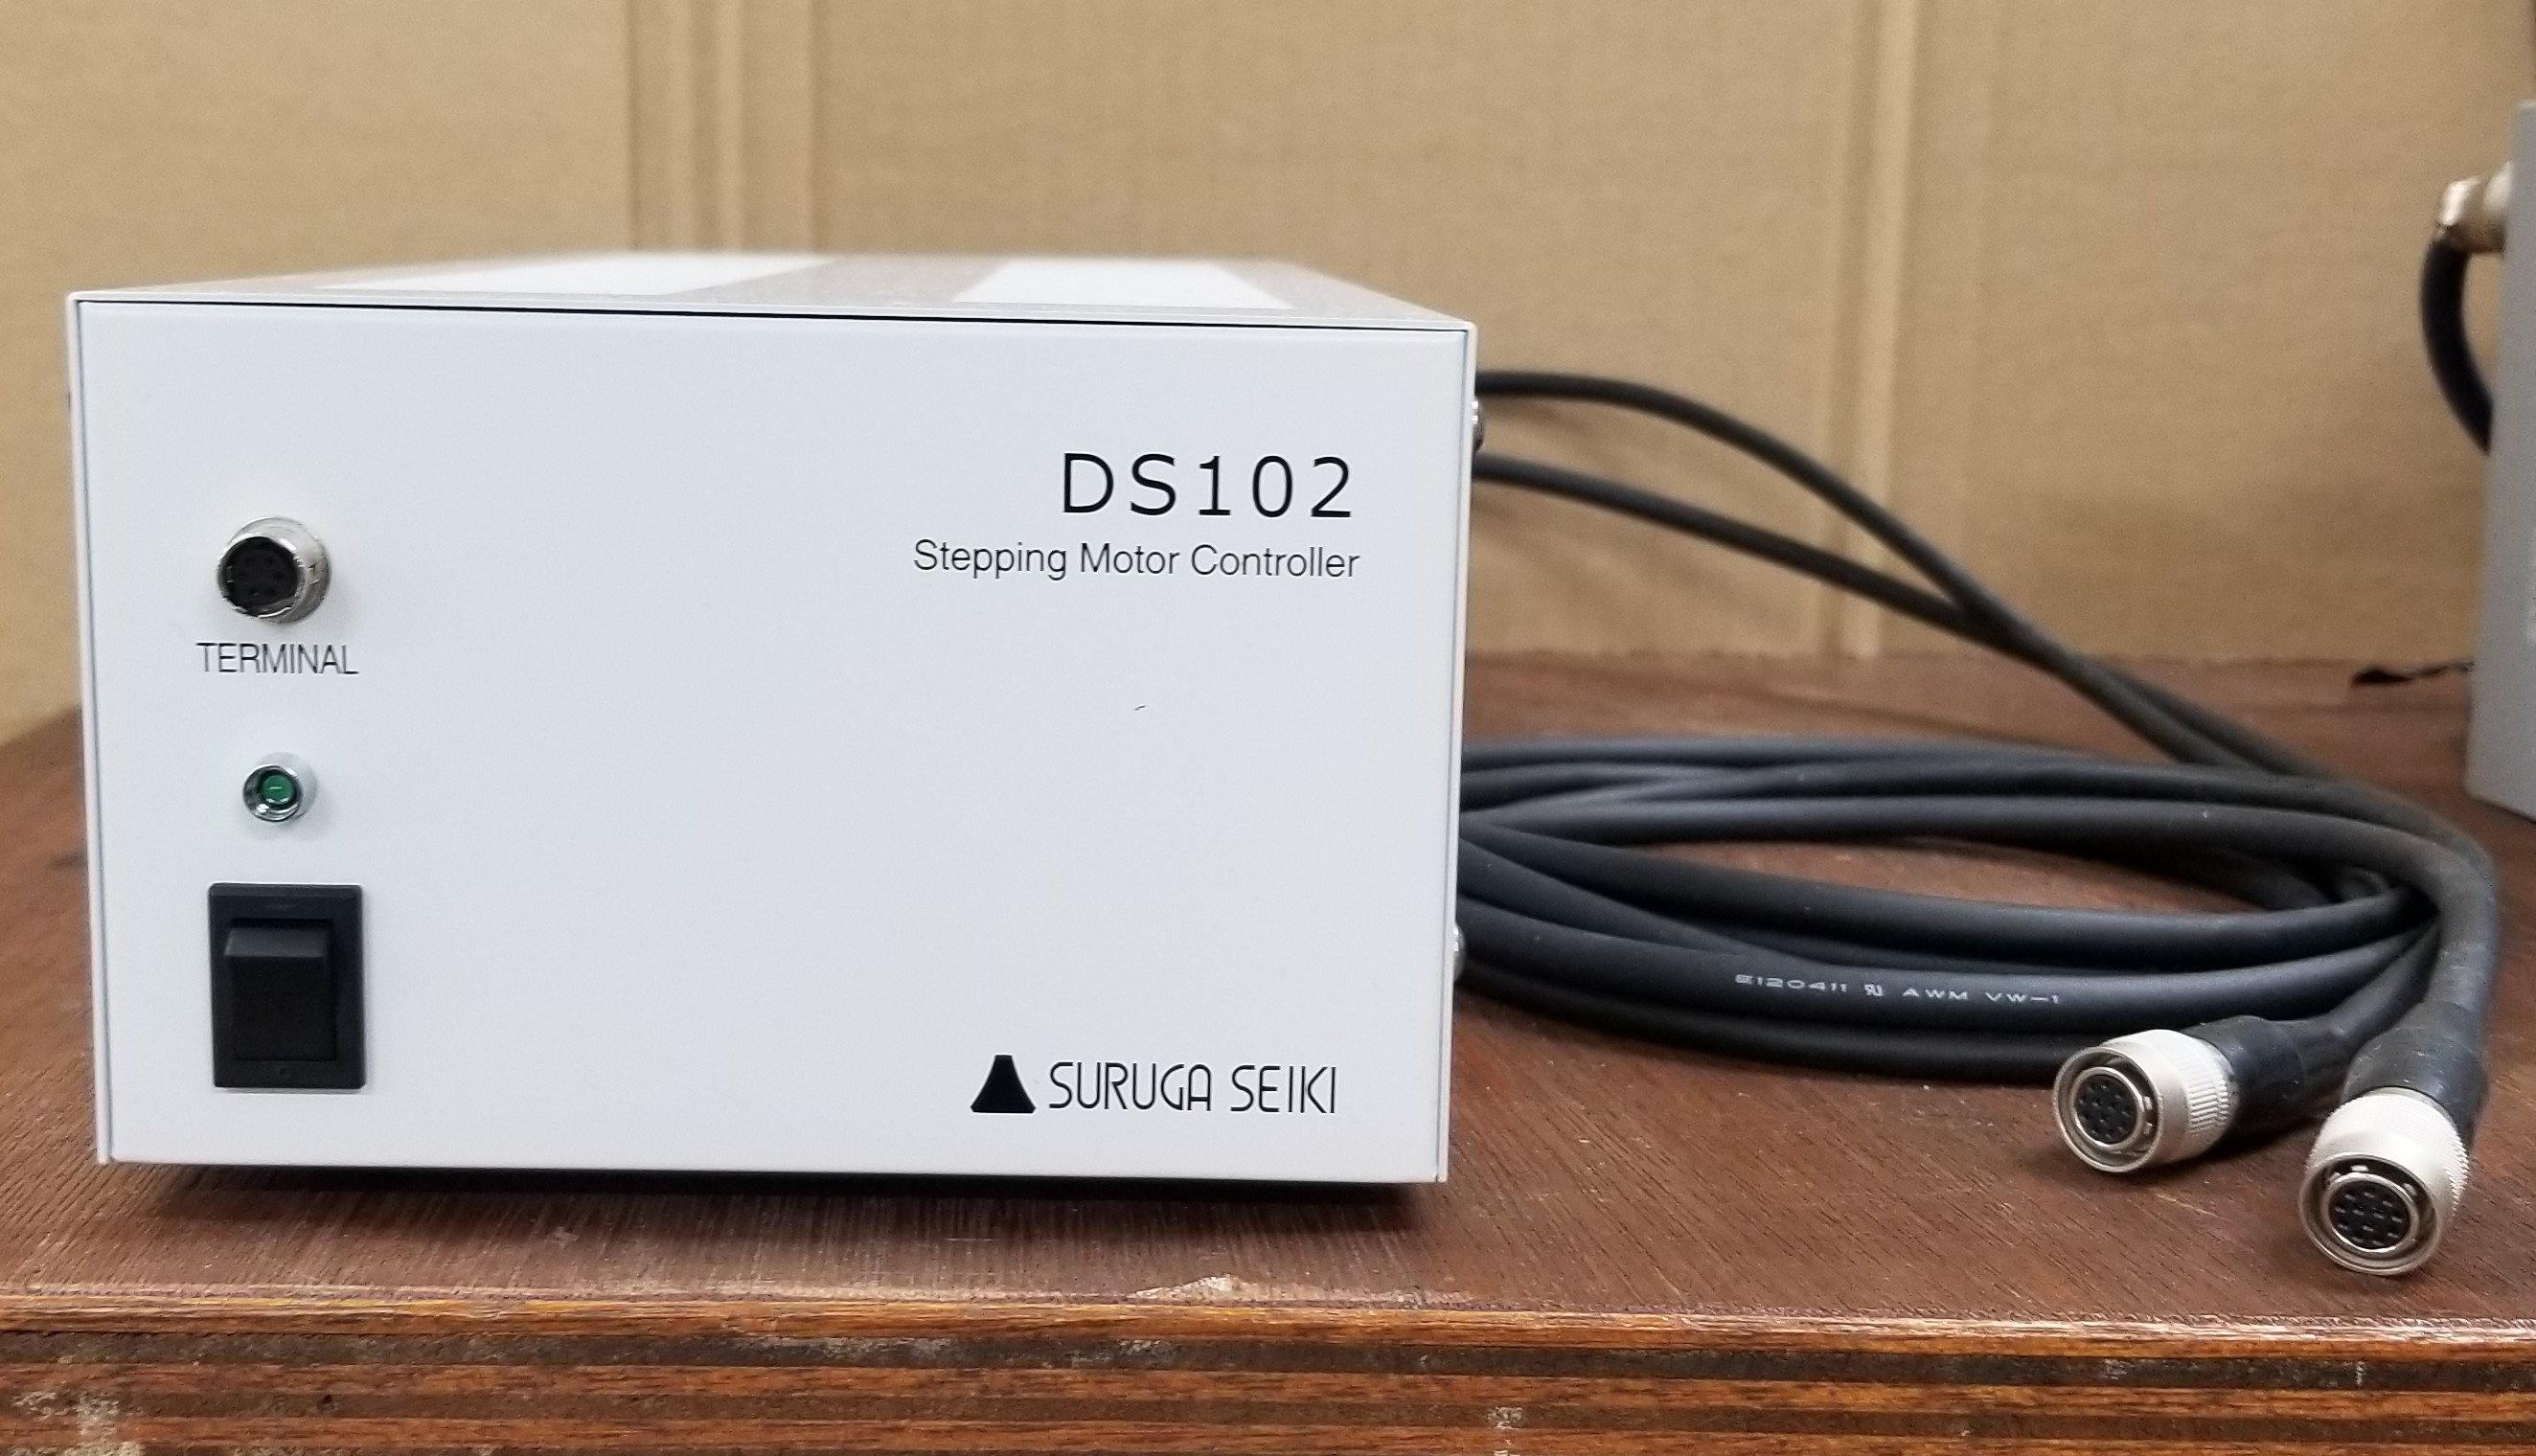
\includegraphics[width=70mm]{images/22-4.png}
        \caption{Stage Controller}
    \end{center}
\end{figure}

\newpage

また,作用力測定装置のひずみセンサ,校正実験装置に取り付けられたロードセルからの出力電圧は
Fig.5に示すロードセルおよびひずみセンサに対応したそれぞれのストレインアンプを通して,
データロガーへと送られ,データロガーに接続されたPCへと保存される.
ロードセルの接続されるストレインアンプ(灰,2個)は,ミネベアミツミ製 動ひずみ測定器(DSA-631),
ひずみセンサの接続されるストレイアンプ(黒,1個)は,ミネベアミツミ製 動ひずみ測定器(DSA-605C),
データロガーには,GRAPHTEC製 高電圧高速 4チャンネルロガー(GL2000) を使用している.
また,Fig.6に本研究で使用した実験装置について,概略図を示す.

\begin{figure}[htbp]
    \footnotesize
    \begin{center}
        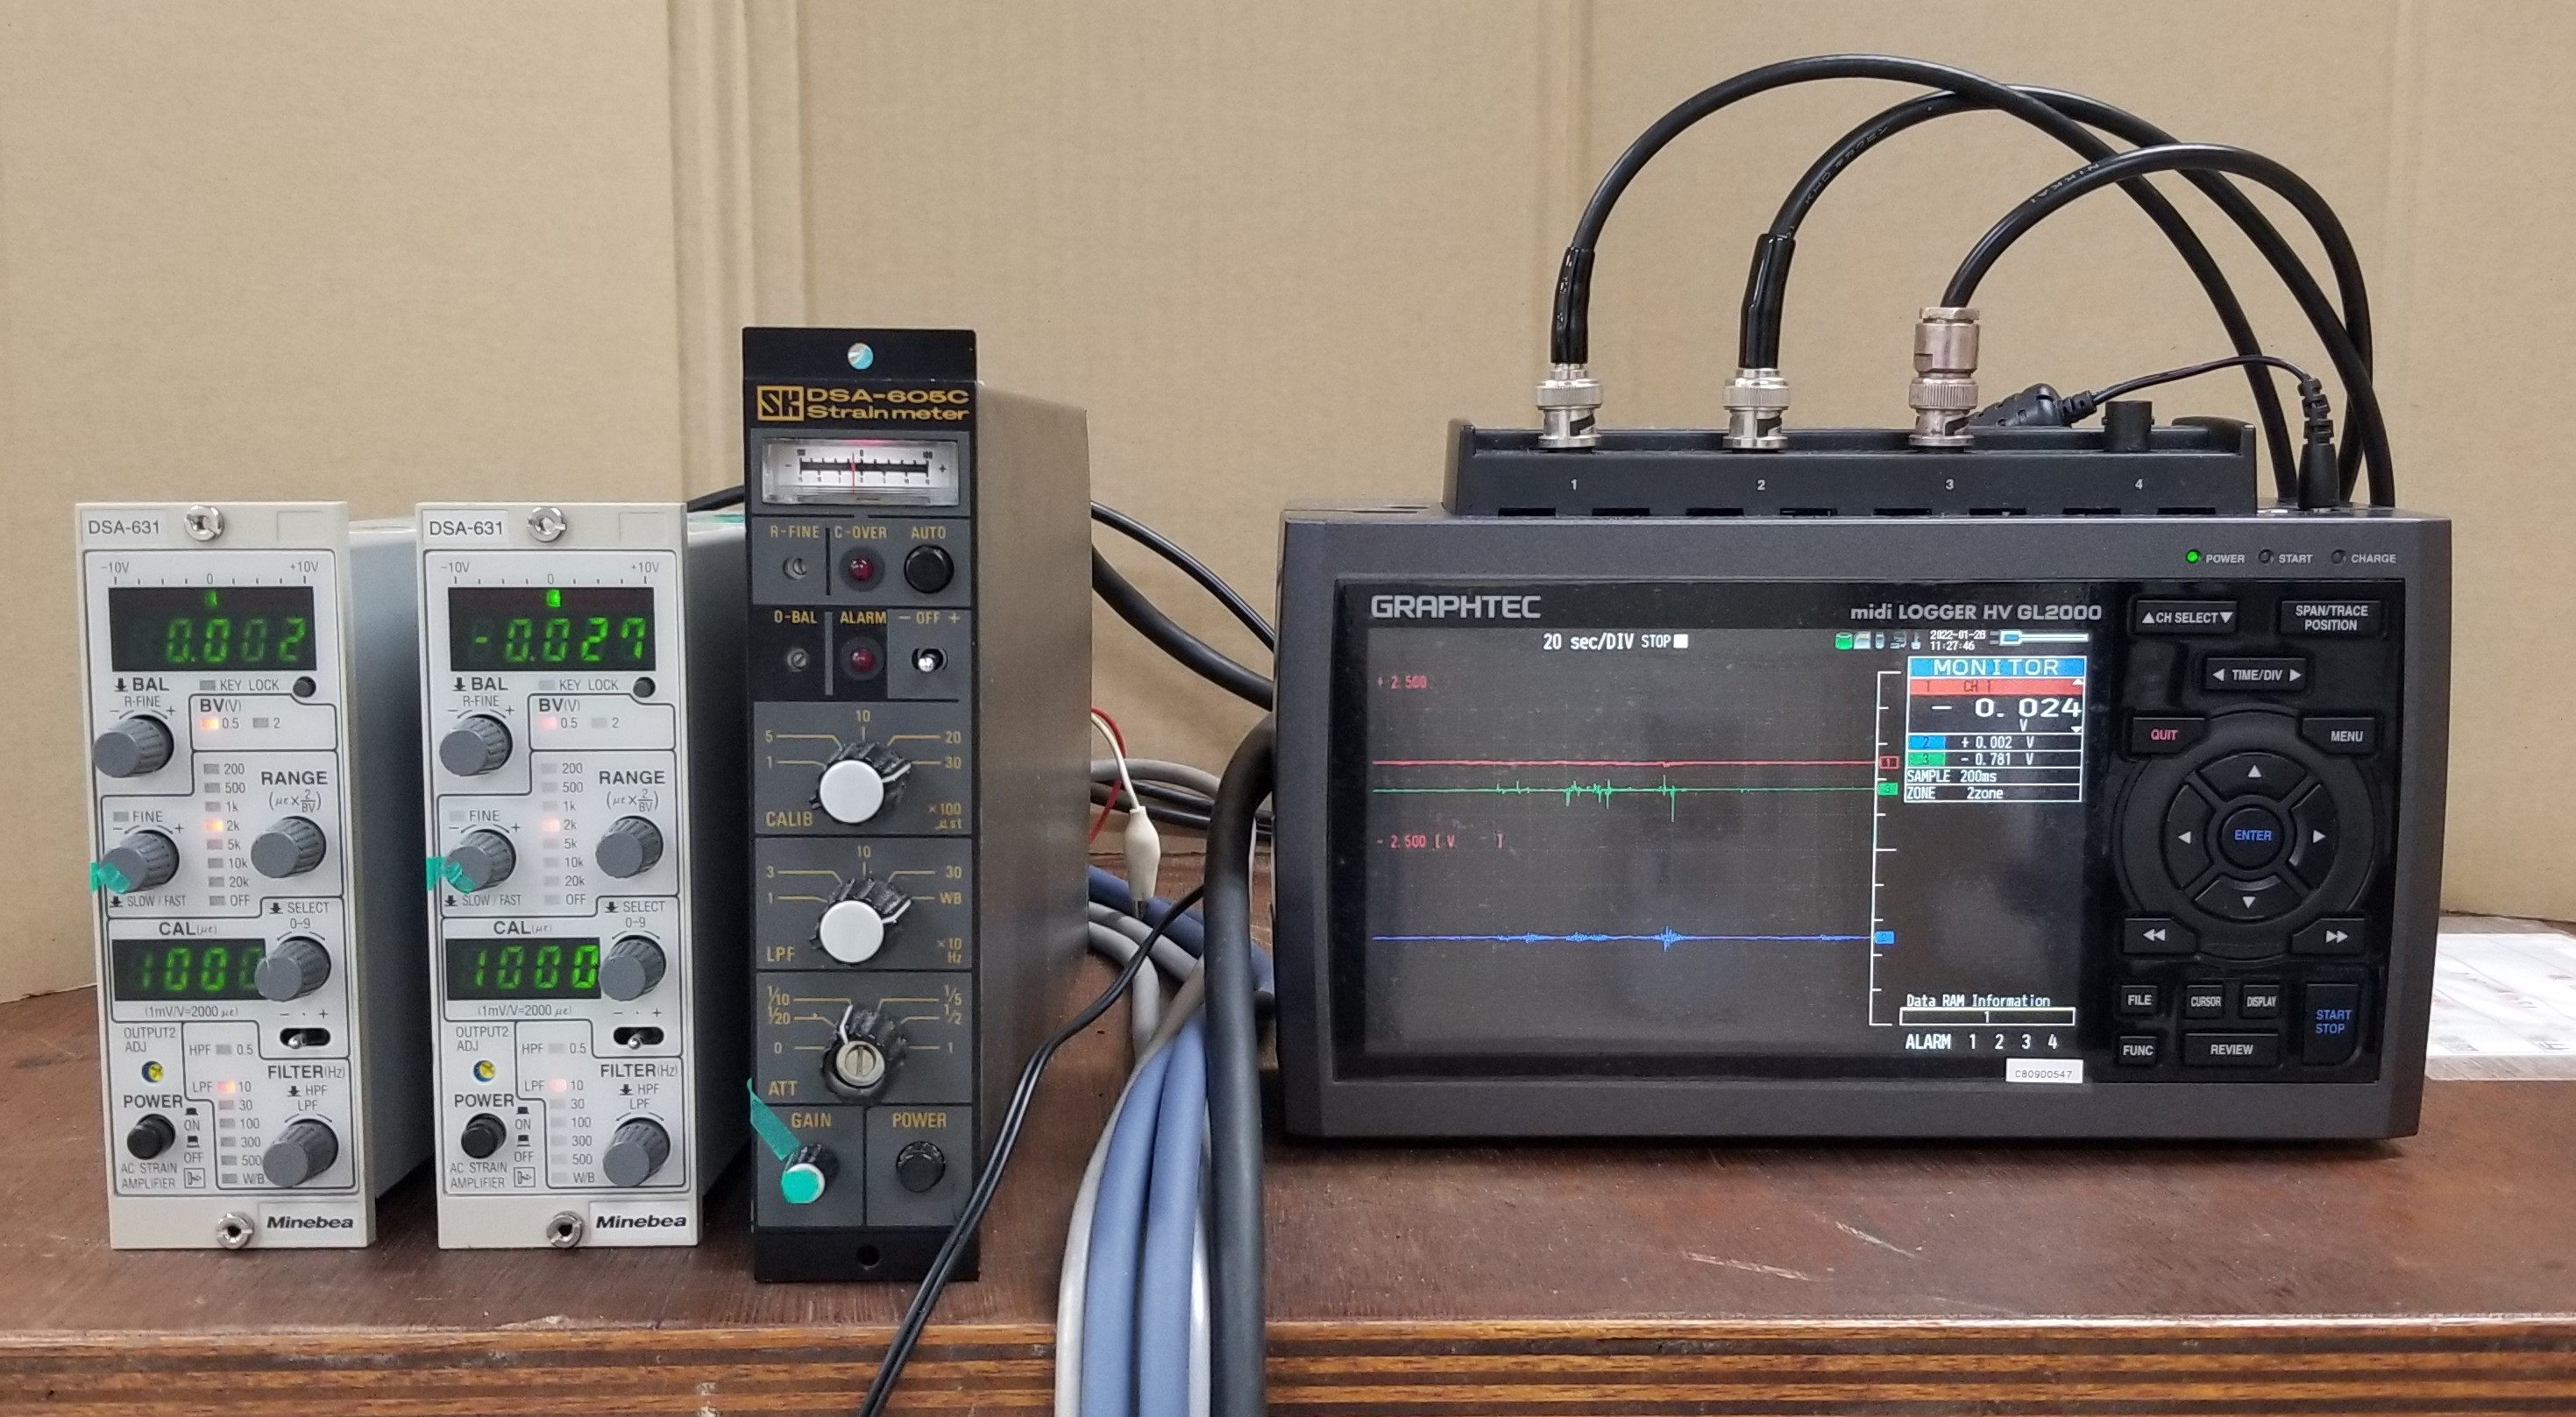
\includegraphics[width=80mm]{images/22-5.png}
        \caption{Strain Amplilifiers and data logger}
        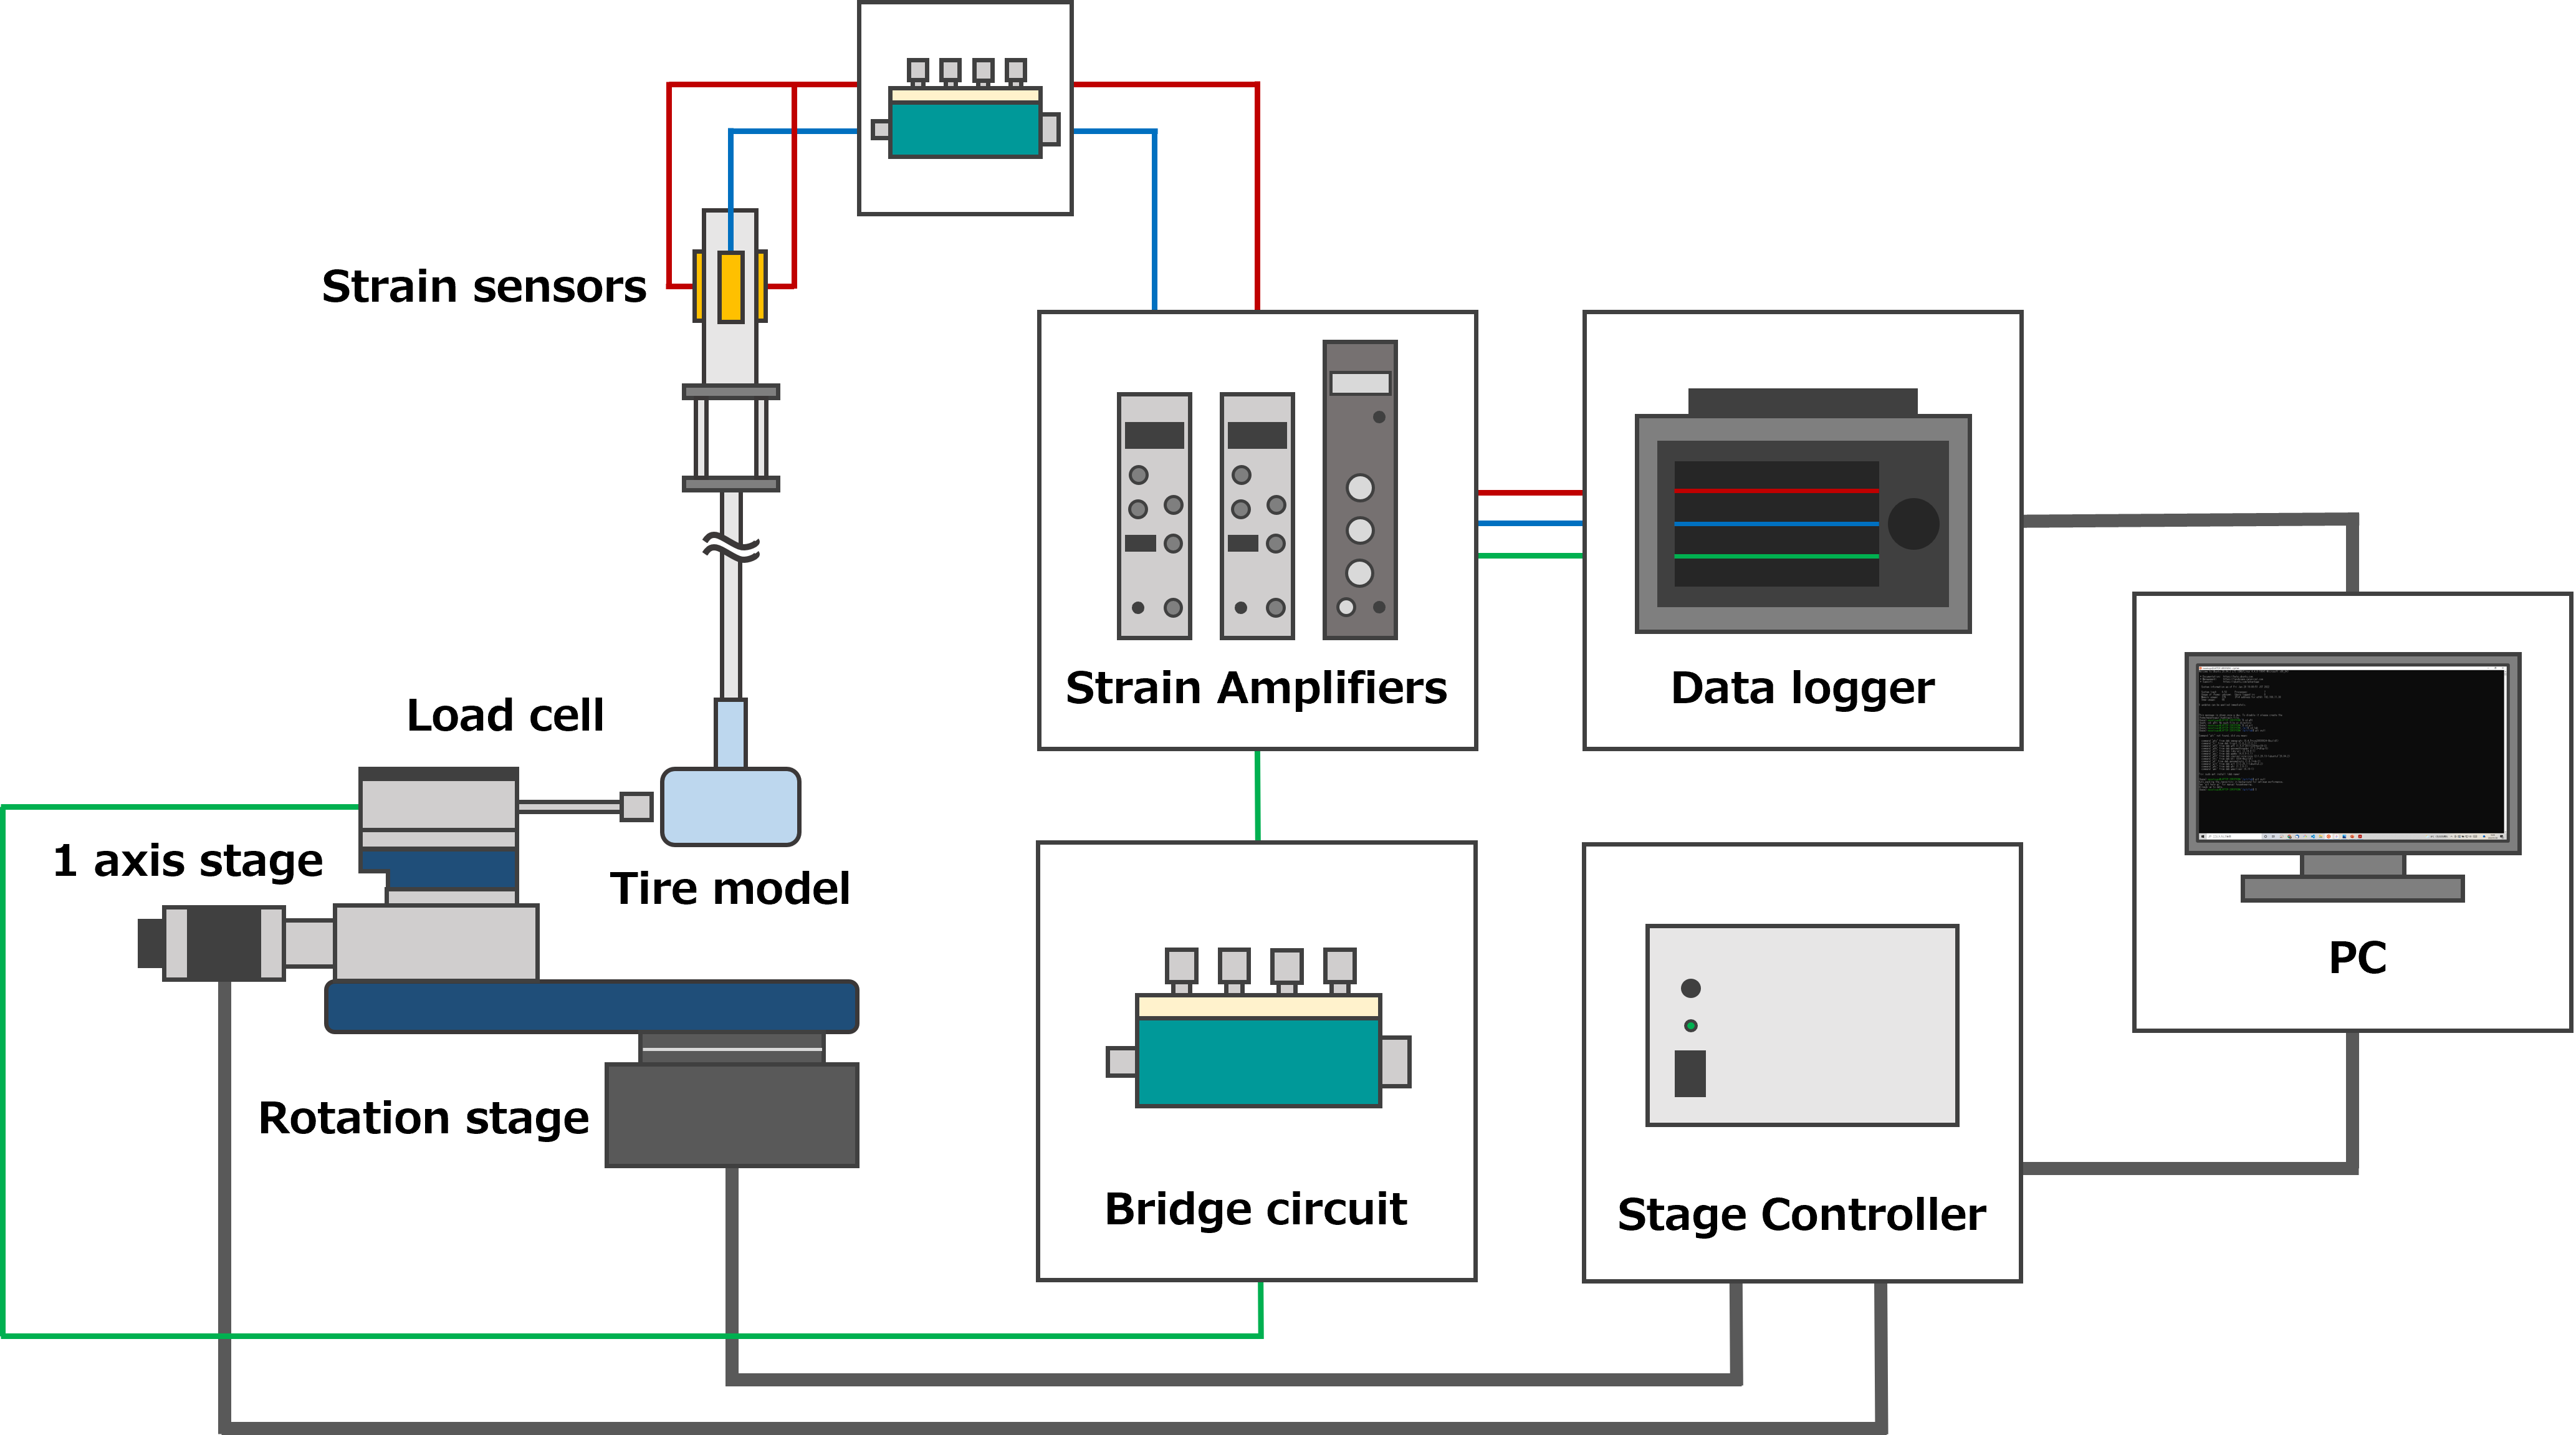
\includegraphics[width=140mm]{images/22-6.png}
        \caption{Schematic of experimental system}
    \end{center}
\end{figure}